%%%%%%%%%%%%%%%
%
% $Autor: Wings $
% $Datum: 2020-01-29 07:55:27Z $
% $Pfad: General/SensorAPDS9960.tex
% $Version: 1785 $
%
%
%%%%%%%%%%%%%%%

\chapter{Sensormodul APDS-9960 for Gesture, Proximity, and Color Detection}

The APDS-9960 sensor, integrated on the Arduino Nano 33 BLE Sense, is a multifunctional optical sensor used for gesture recognition, ambient light detection, color sensing, and proximity measurement. The sensor uses an I²C interface for communication and comes equipped with an additional infrared LED.
\cite{Avago:2015}

\section{General Information}

The general functionality of a color sensor is based on the reflection of white light from the object to be measured. White light contains wavelengths that cover the entire visible spectrum (p. 189 \cite{Rybach:2013}). Due to the molecular structure of the object or chemical processes, such as photosynthesis, certain wavelengths are absorbed while others are reflected. The reflected light rays that reach the color sensor are spectrally selected by color filters or a diffraction grating (p. 459 \cite{Hering:2018}). 

\textbf{Color filters}: By using parallel red, green, and blue color filters, the intensities of the RGB components are evaluated by three photodiodes behind the filters (p. 459 \cite{Hering:2018}).

\textbf{Diffraction grating}: As light passes through a diffraction grating, the physical diffraction effect occurs. This effect, due to the varying wavelengths of light, produces an interference pattern that enables the spectral decomposition of the light. The spectrum of the incoming light is spatially dispersed, similar to the refraction in a prism (p. 208 ff. \cite{Rybach:2013}). The intensity of the color components can be measured by an array of spatially arranged photodiodes. Diffraction gratings offer higher resolution than color filters (p. 459 \cite{Hering:2018}).

Photodiodes are semiconductors that generate electrical energy through the internal photoelectric effect (p. 220 \cite{Rybach:2013}). The signal from the photodiodes is amplified and stored in a data register through analog-to-digital conversion. The measurement is taken over a specific period. By accumulating the RGB data, the measured color can finally be determined \cite{Avago:2015}. 

Color sensors are typically used in image processing and quality control applications \cite{Avago:2015}.

\section{Functionality of the APDS-9960}

\begin{center}    
	\begin{tikzpicture}
		\node at (0,0) (Board) {
\includegraphics{Arduino/Nano33BLE/Nano33BLESense}};
		
		\fill[gray, opacity=0.7] (-6,-2.4) rectangle (6,2.4);
		
		\coordinate (A) at (-1,0.4);
		\coordinate (B) at (0.2,-0.2);    
		\begin{scope}
			\clip (A) rectangle (B);
			\node at (0,0) (Board) {
\includegraphics{Arduino/Nano33BLE/Nano33BLESense}};
		\end{scope}
		\draw[yellow,line width=2pt] (A) rectangle (B);
	\end{tikzpicture}    
	
	\captionof{figure}{Arduino Nano 33 BLE Sense's APDS-9960}
	\label{fig:5.1}
\end{center}

The sensor is located centrally on the Arduino Nano 33 BLE Sense, as indicated in the figure \ref{fig:5.1}.

\subsection{Function of the Color Sensor}

As shown in Figure \ref{fig:SchematicColorSensor}, the incoming light first passes through UV and IR filters. It is then separated into its red, green, blue, and unfiltered components by color filters. These filtered components are subsequently converted from analog to digital units, as described below.

\begin{center}
	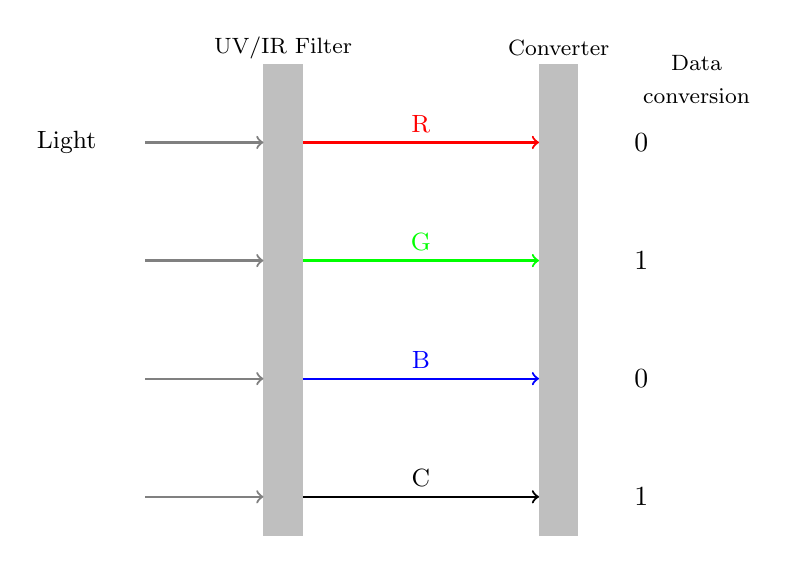
\begin{tikzpicture}
		
		% UV/IR Filter and Converter rectangles
		\fill[gray!50] (2, -2.5) rectangle (2.5, 3.5);
		\fill[gray!50] (5.5, -2.5) rectangle (6, 3.5);
		
		% Labels
		\node at (-0.5, 2.5) {\small Light};
		\node at (2.25, 3.7) {\footnotesize UV/IR Filter};
		\node at (5.75, 3.7) {\footnotesize Converter};
		\node[align=center] at (7.5, 3.3) {\footnotesize Data \\ \footnotesize conversion};
		
		% Arrows for light input
		\draw[->, thick, gray] (0.5, 2.5) -- (2, 2.5);
		\draw[->, thick, gray] (0.5, 1) -- (2, 1);
		\draw[->, thick, gray] (0.5, -0.5) -- (2, -0.5);
		\draw[->, thick, gray] (0.5, -2) -- (2, -2);
		
		% Color-coded arrows
		\draw[->, thick, red] (2.5, 2.5) -- (5.5, 2.5) node[midway, above] {\small R};
		\draw[->, thick, green] (2.5, 1) -- (5.5, 1) node[midway, above] {\small G};
		\draw[->, thick, blue] (2.5, -0.5) -- (5.5, -0.5) node[midway, above] {\small B};
		\draw[->, thick, black] (2.5, -2) -- (5.5, -2) node[midway, above] {\small C};
		
		% Data conversion outputs
		\node at (6.8, 2.5) {0};
		\node at (6.8, 1) {1};
		\node at (6.8, -0.5) {0};
		\node at (6.8, -2) {1};
	\end{tikzpicture}
	
		\captionof{figure}{Schematic of the main function of a color sensor}
	\label{fig:SchematicColorSensor}
\end{center}

The block diagram \ref{fig:FunctionalBlockDiagram} shows the processing flow of the APDS-9660 from light detection to communication via the I²C protocol with the Arduino. The individual steps are explained as follows:

\tikzstyle{block} = [rectangle, draw, minimum width=3.5cm, minimum height=1.2cm, text centered, text width=3.5cm]
\tikzstyle{smallblock} = [rectangle, draw, minimum width=3.5cm, minimum height=1.2cm, text centered]
\tikzstyle{arrow} = [thick,->,>=stealth]
\tikzstyle{sensor} = [draw, isosceles triangle, isosceles triangle apex angle=60, shape border rotate=-90, minimum height=1.5cm, minimum width=1.5cm, text centered]

\begin{center}
	\begin{tikzpicture}[node distance=2.5cm, scale=0.5, every node/.style={transform shape}]
		
		% Sensors
		\node (clear) [sensor] {Clear};
		\node (red) [sensor, below of=clear] {Red};
		\node (green) [sensor, below of=red] {Green};
		\node (blue) [sensor, below of=green] {Blue};
		
		% RGBC + ALS
		\node (rgbc_als) [block, right of=red, xshift=3cm] {RGBC \\ ALS};
		
		% MUX
		\node (mux) [smallblock, right of=rgbc_als, xshift=3cm] {MUX};
		
		% ADC
		\node (adc) [smallblock, right of=mux, xshift=3cm] {ADC};
		
		% FIFO + Threshold Control
		\node (fifo) [block, right of=adc, xshift=3.5cm] {32 x 4 Byte FIFO \\ Threshold Control};
		
		% I2C Interface
		\node (i2c) [block, above of=fifo, yshift=2cm] {I\textsuperscript{2}C Interface};
		
		% Interrupt
		\node (interrupt) [smallblock, below of=fifo, yshift=-2cm] {Interrupt};
		
		% Connections
		\draw [arrow] (clear) -- (rgbc_als);
		\draw [arrow] (red) -- (rgbc_als);
		\draw [arrow] (green) -- (rgbc_als);
		\draw [arrow] (blue) -- (rgbc_als);
		\draw [arrow] (rgbc_als) -- (mux);
		\draw [arrow] (mux) -- (adc);
		\draw [arrow] (adc) -- (fifo);
		\draw [arrow] (fifo) -- (i2c);
		\draw [arrow] (fifo) -- (interrupt);
		\draw [arrow] (i2c) -- ++(2.5cm,0) node[right] {SCL};
		\draw [arrow] (i2c) -- ++(2.5cm,-1.5cm) node[right] {SDA};
		\draw [arrow] (interrupt) -- ++(2.5cm,0) node[right] {INT};
		
	\end{tikzpicture}
	
	\captionof{figure}{Functional Block Diagram}
	\label{fig:FunctionalBlockDiagram}
\end{center}

The photodiodes convert the intensities of the color components of the filtered light and the total light into electrical signals.
These RGBC and ALS signals are forwarded to the next processing stage using the multiplexer (MUX). 

The MUX allows for the sequential processing of the color signals, as the ADC (Analog-to-Digital Converter) can only process one signal at a time.
The ADC converts the analog signal selected by the MUX into a digital value. This conversion is necessary to make the signal suitable for digital processing and transmission.

The digital value is stored in a FIFO (First in-First out) data register, which can store up to 32 data values (4 bytes each). A threshold controller monitors the data and triggers an interrupt when defined limits are reached. The detailed process is explained in Chapter Data Processing \ref{chap:Data Processing}.

The stored data is transmitted to the Arduino via an I²C bus. The I²C bus uses two lines: the SCL (Serial Clock Line) for the clock and the SDA (Serial Data Line) for data transmission. The detailed functioning of the I²C bus is explained in Chapter \ref{chap:Protokoll I²C} Protokoll I²C.
\cite{Avago:2015}.

\subsubsection{Data Processing}
\label{chap:Data Processing}

The color detection begins at the photodiodes with RGBC detection and ends with 16-bit values stored in the RGBC data registers. The signal from the photodiode array is accumulated over a period defined by the value in the ATIME register (ALS ADC Integration Time) before the results are transferred to the RGBCDATA registers. The gain factor can be set from 1x to 64x, which is controlled via the CONTROL<AGAIN> bit (ALS Gain Control). Performance parameters such as accuracy, resolution, conversion speed, and energy consumption can be adjusted to meet the application requirements.

Between measurements, a customizable, energy-efficient waiting period is maintained, the duration of which is determined by the control bits WEN (Wait Enable), WTIME (Wait Time), and WLONG (Wait Long Enable). The waiting time can range from 0 seconds to a maximum of 8.54 seconds.

An interrupt is triggered when the clear channel values exceed the thresholds defined in the AILTL/AIHTL (ALS low threshold, lower byte/ALS high threshold, lower byte) or AILTH/AIHTH (ALS low threshold, upper byte/ALS high threshold, upper byte) threshold registers. To avoid unwanted or false interrupts, a persistence filter is integrated, ensuring that an interrupt is triggered only when a defined number of consecutive values fall outside the thresholds. This threshold is set in the APERS register (ALS Interrupt Persistence). If a value is within the thresholds, the persistence counter is reset. If the analog circuit is saturated, the ASAT bit is set, indicating potentially inaccurate RGBCDATA results. The AINT (ALS Interrupt) and CPSAT (Clear Diode Saturation) bits can be queried at any time via I²C. However, for AINT to trigger a hardware interrupt on the INT pin, the AIEN bit (ALS Interrupt Enable) must be set. Saturation of the analog-to-digital converter can be detected via the CPSAT bit; to enable this function, the CPSIEN bit (Clear Diode Saturation Interrupt Enable) must be set. The AVALID bit (ALS Valid) is reset by reading the RGBCDATA. ASAT and AINT can be reset via the CICLEAR (Clear Channel Interrupt Clear) or AICLEAR (All Non-Gesture Interrupt Clear) bits.

The RGBC results can be used to determine the color temperature in Kelvin or the ambient light intensity in Lux.

\cite{Avago:2015}

\subsection{Function of the Ambient Light Sensor}

The ambient light sensor (ALS) of the APDS-9960 works with the same photodiode array and measures the intensity of the ambient light. For this purpose, the UV and IR light filters are installed in front of the photodiodes to ensure accurate measurements of visible light. The sensor converts the measured light intensity into 16-bit data, which enables high resolution and accuracy. A function of programmable gain and customizable integration time ensures that the sensor can operate accurately in different lighting conditions, such as dim or very bright light.
\medskip
Another important feature of the sensor is its ability to correctly detect the intensity of ambient light even behind dark glass, which is particularly useful for devices with tinted covers.
\smallskip
\cite{Avago:2015}

\subsection{Function of the Gesture Detection Sensor}

The gesture recognition of the APDS-9960 is based on four additional angled photodiodes (top, bottom, left, right), which detect reflected infrared light (IR) from the integrated IR-LED. By analyzing the reflection, which measures direction-dependent changes using the photodiodes, the sensor can recognize movements and gestures such as swiping motions in different directions (e.g., up, down, left, right). The sensor converts this information into digital data, such as speed, direction, and distance of the movement. The 32-record FIFO register allows the sensor to temporarily store motion data, ensuring continuous processing.
\smallskip
\cite{Avago:2015}

\subsection{Function of the Proximity Sensor}

The proximity sensor is part of the gesture detection sensor and detects top-bottom gestures based on the temporal change in the measured distance. The proximity detection measures the distance between the sensor and an object by capturing the reflected IR light. The integrated IR LED emits light, which is measured by the same photodiodes as in gesture detection. The stronger the reflection, the closer the object is. The proximity sensor can also detect events such as the approach or withdrawal of an object and trigger corresponding interrupts when predefined thresholds are exceeded. To ensure reliable measurements, the sensor compensates for unwanted reflections by adjusting offset values and suppresses interference from ambient light.
\smallskip
\cite{Avago:2015}

\section{Key Technical Specifications}
\label{chap:Specification}

\subsection*{Power Supply}
\begin{itemize}
	\item Supply Voltage: 2.4 V to 3.6 V
	\item Maximum Voltage: 3.8 V
\end{itemize}

\subsection*{Power Consumption}
\begin{itemize}
	\item Active ALS Mode (Ambient Light Sensor): 200-250 µA
	\item Proximity and Gesture Modes: 790 µA (without LED)
	\item Sleep Mode: 1-10 µA
\end{itemize}

\subsection*{Temperature}
\begin{itemize}
	\item Operating Temperature Range: -30°C to +85°C
	\item Storage Temperature Range: -40°C to +85°C
\end{itemize}

\subsection*{Optical Properties}
\begin{itemize}
	\item LED Wavelength (max.): 950 nm
	\item LED Drive Current:
	\begin{itemize}
		\item 100 mA (Standard), 50 mA, 25 mA, 12.5 mA
		\item LED Boost Option: 100\%, 150\%, 200\%, 300\% (adjustable current boost)
	\end{itemize}
	\item Max Detection Distance for Color, Proximity and Gesture Sensor 0mm to 100mm
\end{itemize}

\subsection*{Proximity Sensor}
\begin{itemize}
	\item Pulse Width for Proximity Measurement: 4 µs to 32 µs
\end{itemize}

\subsection*{Gesture Sensor}
\begin{itemize}
	\item LED Pulse Count: 1 to 64 pulses
\end{itemize}

\subsection*{Connections}
\begin{itemize}
	\item I2C Communication:
	\begin{itemize}
		\item Data Rates: Up to 400 kHz
		\item Pins:
		\begin{itemize}
			\item SDA (I2C Data)
			\item SCL (I2C Clock)
			\item INT (Interrupt, Open Drain, Active Low)
			\item LDR (LED Driver Input)
		\end{itemize}
	\end{itemize}
\end{itemize}

\subsection*{Dimensions}
\begin{itemize}
	\item Length: 3.94mm
	\item Width: 2.36mm
	\item Height: 1.35mm
\end{itemize}

\cite{Avago:2015}


\section{Library}

In the case of the APDS-9960 sensor, Arduino provides a library \FILE{Arduino\_APDS9960} for calling functions related to color detection, distance measurement, or gesture recognition.

The library for the sensor is \FILE{Arduino\_APDS9960}. This allows measuring gestures, colors, light intensity, and distances with the sensor. Communication between the Arduino Nano 33 BLE Sense's chip and the APDS-9960 module occurs via an internal I²C interface \cite{Avago:2015}.

The library is included by using the command \PYTHON{\#include <Arduino\_APDS9960.h>}.

The current version is 1.0.4 (as of 19.09.2024).




\subsection{Installation of APDS-9960 Library}

The library is installed as follows:

\menu[,]{Tools,Manage Libraries...}

\begin{enumerate}
	\item Open the Arduino IDE and navigate to \menu[,]{Tools,Manage Libraries...}.
	\item In the Library Manager, use the search bar to look for "Arduino\_APDS9960".
	\item Several libraries will be displayed. Select the library titled "Arduino\_APDS9960" by Arduino and click \textit{Install}.
	\item Once installed, the IDE will show a message in the console confirming the installation. The "Install" button will also change to "Remove", indicating the library is ready for use.
\end{enumerate}

\subsection{Functions}

\begin{itemize}
	\item \PYTHON{begin()}: The \PYTHON{begin()} method activates and initializes the APDS9960 sensor. It is typically called during the \PYTHON{setup\{\}} phase.
	
	\medskip
	
	\begin{itemize}
		\item Return value \PYTHON{TRUE}: Initialization was successful.
		\item Return value \PYTHON{FALSE}: Initialization failed.
	\end{itemize}
	
	\item \PYTHON{end()}: The \PYTHON{end()} method deactivates the APDS9960 sensor.
	
	
	\item \PYTHON{colorAvailable()}: This method checks if color data is available to be retrieved.
	
	\medskip
	
	\begin{itemize}
		\item Return value \PYTHON{TRUE}: Color data is available.
		\item Return value \PYTHON{FALSE}: No color data is available.
	\end{itemize}
	
	\item \PYTHON{readColor(...)}: This method retrieves the color values from the sensor.
	
	It can either read just the color values or the color values along with the ambient light intensity.
	
	\medskip
	
	To read only the color values:
	
	\PYTHON{int r, g, b;}
	
	\PYTHON{APDS.readColor(r, g, b);}
	
	\medskip
	
	The variables \PYTHON{r}, \PYTHON{g}, and \PYTHON{b} will contain the updated color values. The value range is $0, 1, 2, \ldots, 255$.
	
	\medskip
	
	To read both the color values and ambient light intensity:
	
	\PYTHON{int r, g, b, a;} 
	
	\PYTHON{APDS.readColor(r, g, b, a);}
	
	\medskip
	
	The variables \PYTHON{r}, \PYTHON{g}, and \PYTHON{b} will contain the updated color values, while \PYTHON{a} will contain the ambient light intensity. The value range is $0, 1, 2, \ldots, 255$.
	
	\item \PYTHON{proximityAvailable()}: This method checks if proximity data is available.
	
	\medskip
	
	\begin{itemize}
		\item Return value \PYTHON{TRUE}: Proximity data is available.
		\item Return value \PYTHON{FALSE}: No proximity data is available.
	\end{itemize}
	
	\item \PYTHON{readProximity()}: This method reads the proximity value.
	
	\medskip
	
	\begin{itemize}
		\item Return value \PYTHON{int proximity = APDS.readProximity()}: Returns the proximity value.
		\item Return value \PYTHON{-1}: Proximity could not be determined.
	\end{itemize}
	
	\item \PYTHON{gestureAvailable()}: This method checks if a gesture has been detected.
	
	\medskip
	
	\begin{itemize}
		\item Return value \PYTHON{TRUE}: A gesture has been detected.
		\item Return value \PYTHON{FALSE}: No gesture detected.
	\end{itemize}
	
	\item \PYTHON{setGestureSensitivity()}: Gesture detection is influenced by lighting conditions, speed, and distance of movement. This function allows you to adjust the sensitivity of gesture recognition. A higher value detects more gestures, but increases the chance of false positives. A lower value reduces the likelihood of detecting gestures.
	
	The valid range is \PYTHON{1} to \PYTHON{100}.
	
	The default value is \PYTHON{80}.
	
	\item \PYTHON{readGesture()}: If a gesture has been detected, it can be retrieved using the \PYTHON{readGesture()} method. The possible return values are:
	
	\begin{itemize}
		\item \PYTHON{GESTURE\_UP}: An upward movement has been detected.
		\item \PYTHON{GESTURE\_DOWN}: A downward movement has been detected.
		\item \PYTHON{GESTURE\_LEFT}: A leftward movement has been detected.
		\item \PYTHON{GESTURE\_RIGHT}: A rightward movement has been detected.
		\item \PYTHON{GESTURE\_NONE}: No gesture has been detected.
	\end{itemize}
	
	\item \PYTHON{setInterruptPin()}: This method sets the pin used to trigger a measurement. The pin is usually detected automatically, but can be set manually using this function.
	
	If \PYTHON{-1} is passed, no pin is connected.
	
	If \PYTHON{0} or a higher value is passed, that pin will be used.
	
	The default value depends on the board.
	
	\item \PYTHON{setLEDBoost(...)}: The sensor includes an infrared LED that can be temporarily boosted to provide higher brightness. It can be set to provide up to 300\% of its normal power. This can be configured using this method.
	
	\medskip
	
	Usage:
	
	\begin{itemize}
		\item \PYTHON{0}: Boost to 100\% (default power).
		\item \PYTHON{1}: Boost to 150\%.
		\item \PYTHON{2}: Boost to 200\%.
		\item \PYTHON{3}: Boost to 300\%.
	\end{itemize}    
	
	\medskip
	
	Return values:
	
	\begin{itemize}
		\item \PYTHON{0}: Failure.
		\item \PYTHON{1}: Success.
	\end{itemize}
\end{itemize}

\cite{ArduinoAPDS9960:2024}


\section{Simple Function Tests}

The following code examples can be used to test and try out all functions of the APDS-9960.

\subsection{Color Detection}

The "Arduino\_APDS9960" library provides an example code demonstrating color detection with the APDS-9960 on an Arduino Nano 33 BLE Sense. The color recognition test program also includes a test of the ambient light sensor, as it utilizes the same sensor technology. The intensities of the color channels are displayed in the Serial Monitor.



\subsection{Color Detection - Manual}

To begin the process of creating the color sensor measurement program, first open the Arduino Cloud Editor. Navigate to the "Libraries" tab and search for the "Arduino\_APDS9960" library. After downloading the library, click on "More info" to get to a github repository where several examples are provided.

Following this, connect the Arduino Nano 33 BLE Sense to your computer. Ensure that the Cloud Editor detects both the board and the corresponding port. If the board is not recognized automatically, follow the instructions to install the necessary plugin, which enables the editor to identify your board. Make sure that you have selected the correct port. Then upload the program to the Arduino. By opening the serial monitor, the measured values are recorded in the Arduino IDE.

\subsection{Color Detection - Code}

First, serial communication is started with \texttt{Serial.begin(9600)} to send data to the computer. The \texttt{APDS.begin()} command initializes the sensor and in the event of a potential error, an error message is output via the serial interface.

\lstinputlisting[firstline=1,lastline=23]{../../Code/Nano33BLESense/Test/TestAPDS9960Color.ino}

The code operates within the \texttt{loop()} function of an Arduino program to continuously read and display color values from the APDS-9960 sensor. Initially, it checks if a color reading is available by using the \texttt{APDS.colorAvailable()} function. If no reading is available, the program briefly pauses for 5 milliseconds to avoid excessive CPU usage. Once a reading is ready, the function \texttt{APDS.readColor(r, g, b)} retrieves the color data and stores the red, green, and blue values in the respective variables. These values are then printed to the Serial Monitor, labeled clearly as "r", "g", and "b". A one-second delay is added before the program repeats the loop, allowing for clear intervals between consecutive readings.

\lstinputlisting[firstline=25,lastline=46]{../../Code/Nano33BLESense/Test/TestAPDS9960Color.ino}

\subsection{Color Detection - File}

The program can be found at \\
\FILE{../../Code/Nano33BLESense/Test/TestAPDS9960Color.ino}.

\subsection{Proximity}

A simple code for testing the proximity sensor is also provided by the library. The proximity sensor is designed for measuring distances of up to 100mm.

\subsection{Proximity - Manual}

Open the Arduino Cloud Editor and navigate to the Libraries tab. In the search bar, search for the "Arduino\_APDS9960" library. Once located, open the Examples section within the library and select the "ProximitySensor" sketch.
\smallskip
Connect the Arduino Nano 33 BLE Sense to the computer. Check that the Cloud Editor recognizes the board by verifying if both the board and port are listed in the dropdown menu.

\subsection{Proximity - Code}

First, serial communication is started with Serial.begin(9600) to send data to the computer. The \texttt{APDS.begin()} command initializes the sensor and in the event of a potential error, an error message is output via the serial interface.

\lstinputlisting[firstline=1,lastline=23]{../../Code/Nano33BLESense/Test/TestAPDS9960Proximity.ino}

The code operates within the \texttt{loop()} function of an Arduino program to continuously read and display proximity values from the APDS-9960 sensor. It begins by checking if a proximity reading is available using the \texttt{APDS.proximityAvailable()} function. If a reading is ready, the function \texttt{APDS.readProximity()} retrieves the proximity value, where 0 indicates a close object, 255 indicates a distant object, and -1 signals an error in reading. This proximity value is then printed to the Serial Monitor. A delay of 100 milliseconds is added before the program repeats the loop, ensuring a brief interval between consecutive readings.

\lstinputlisting[firstline=25,lastline=40]{../../Code/Nano33BLESense/Test/TestAPDS9960Proximity.ino}

\subsection{Proximity - File}

The program can be found at \\
\FILE{../../Code/Nano33BLESense/Test/TestAPDS9960Proximity.ino}.

\subsection{Gesture Detection}

The library also provides an example code demonstrating gesture detection with the APDS-9960 on an Arduino Nano 33 BLE Sense. Some LED feedback signals have been programmed to provide quick visual feedback.

\subsection{Gesture Detection - Manual}

Open the Arduino Cloud Editor and navigate to the Libraries tab. In the search bar, search for the "Arduino\_APDS9960" library. Once located, open the Examples section within the library and select the "GestureSensor" sketch.
\smallskip
Connect the Arduino Nano 33 BLE Sense to the computer. Check that the Cloud Editor recognizes the board by verifying if both the board and port are listed in the dropdown menu.

\subsection{Gesture Detection - Code}

In this code example, the APDS-9960 library is integrated first and then the setup is created.
In addition, the LED pins are configured so that they behave as outputs.

\lstinputlisting[firstline=1,lastline=25]{../../Code/Nano33BLESense/Test/TestAPDS9960Gesture.ino}

 After that, \texttt{Serial} communication is initialized, and the program verifies whether the sensor is correctly initialized using \texttt{APDS.begin()}. If initialization fails, an error message is printed. The gesture sensitivity can be adjusted via \texttt{APDS.setGestureSensitivity(value)}, where values range from 1 to 100, affecting detection accuracy and sensitivity. The program sets a default sensitivity and signals the start of gesture detection by turning off the RGB LEDs with \texttt{digitalWrite(LEDR, HIGH)}, \texttt{digitalWrite(LEDG, HIGH)}, and \texttt{digitalWrite(LEDB, HIGH)}.

In the \texttt{loop()} function, the code continuously checks for available gestures using \texttt{APDS.gestureAvailable()}. When a gesture is detected, it is read using \texttt{APDS.readGesture()} and interpreted within a \texttt{switch} statement. Each gesture corresponds to specific LED behavior:

\begin{itemize}
	\item \texttt{GESTURE\_UP}: The red LED is briefly turned on, then off after a 1-second delay.
	\item \texttt{GESTURE\_DOWN}: The green LED is briefly turned on, then off after a 1-second delay.
	\item \texttt{GESTURE\_LEFT}: The blue LED is briefly turned on, then off after a 1-second delay.
	\item \texttt{GESTURE\_RIGHT}: All LEDs are turned on simultaneously, then off after a 1-second delay.
\end{itemize}

The \texttt{default} case ensures no action if an undefined gesture is detected.

\lstinputlisting[firstline=26,lastline=79]{../../Code/Nano33BLESense/Test/TestAPDS9960Gesture.ino}


\subsection{Gesture Detection - File}

The program can be found at \\
\FILE{../../Code/Nano33BLESense/Test/TestAPDS9960Gesture.ino}.

\subsection{Troubleshoot}

If the Arduino is connected to the wrong port or there is an accidental interruption of the cable connection, it can lead to communication issues between the Arduino and the computer. This may result in failure to upload code or the inability to establish a proper serial connection. To resolve this, ensure that the correct port is selected in the Arduino IDE under the "Tools" menu, and verify that the USB cable is securely connected. If the problem persists, try reconnecting the cable or using a different USB port to eliminate any potential hardware faults.

\medskip

Errors in color detection can also be caused by insufficient lighting in the room. Please ensure that the environment is bright enough for the color detection function.

\section{Calibration Color Detection}

Due to variations in environmental light conditions and the sensitivity of the sensor, calibration is required to ensure accurate color detection. This section outlines the calibration process using a standard color chart under constant lighting conditions. To carry out the calibration, the Arduino, a connection cable (USB A to USB Micro), and a laptop or computer with the appropriate Arduino development environment are required.

\medskip

The proximity and gesture feature is pre-configured and factory-calibrated to detect proximity and gesture at a distance of 100mm, eliminating the need for customer calibration.
\cite{BroadcomAPDS9960:2024}

\subsection{Calibration Setup}
A standardized color chart is used, which provides reference values for perfect red, green, and blue under constant lighting conditions. The RGB values from the sensor are read as raw, uncalibrated data, which must be normalized to a standard range (0–255) for accurate color detection.

\subsection{Step 1: Measuring Reference Values}
The first step in the calibration process is to measure the raw sensor values for each primary color (red, green, and blue) using the standardized color chart. By placing the color chart in front of the sensor and reading the raw RGB values, we can establish the maximum possible sensor readings for each color channel.

\[
\text{RawRed} = \max(R_{\text{measured}})
\]
\[
\text{RawGreen} = \max(G_{\text{measured}})
\]
\[
\text{RawBlue} = \max(B_{\text{measured}})
\]

These maximum values are obtained by positioning the chart at a fixed distance of one centimeter and ensuring constant light intensity.

\subsection{Step 2: Normalizing the Sensor Values}
Once the maximum sensor readings for red, green, and blue are obtained, the raw sensor data is normalized to a 0-255 scale. This ensures that the sensor's readings correspond to standard RGB values. The following formula is used for normalization:

\[
R_{\text{calibrated}} = \frac{R_{\text{raw}}}{\text{RawRed}} \times 255
\]
\[
G_{\text{calibrated}} = \frac{G_{\text{raw}}}{\text{RawGreen}} \times 255
\]
\[
B_{\text{calibrated}} = \frac{B_{\text{raw}}}{\text{RawBlue}} \times 255
\]

Where:
\begin{itemize}
	\item $R_{\text{raw}}, G_{\text{raw}}, B_{\text{raw}}$ are the raw sensor values for each channel.
	\item $\text{RawRed}, \text{RawGreen}, \text{RawBlue}$ are the maximum measured values from the standard color chart.
\end{itemize}

\subsection{Step 3: Implementing the Calibration in Code}
The normalization process is implemented directly in the Arduino code to adjust the sensor's readings. To begin calibration, open the Serial Monitor, enter "OK" in the command line, and press Enter to confirm. The following steps will then be explained through text output.
\medskip
After the user initiates the calibration by typing "OK" into the serial monitor, the program starts. The program then guides the user through the calibration of red, green, and blue colors, with each phase confirmed by entering "OK". The pins for the RGB LEDs are defined, and variables store the maximum calibration values for each color. Status variables control the sequence, ensuring each phase is completed before moving to the next. These maximum values are later used for accurate color detection in the Application code.

\lstinputlisting[firstline=1,lastline=28]{../../Code/Nano33BLESense/APDS9960Calibration/APDS9960Calibration.ino}

The following code section begins by initializing serial communication at a baud rate of 9600, enabling interaction through the serial monitor. Next, it sets the RGB LED pins as outputs and turns on all LEDs to create white light, which helps capture accurate color measurements. The code then initializes the APDS-9960 sensor, checking for successful setup. If the sensor fails to initialize, an error message is printed, and the program halts. If successful, a message confirms initialization and prompts the user to type "OK" in the serial monitor to proceed with the calibration process explanation.

\lstinputlisting[firstline=30,lastline=51]{../../Code/Nano33BLESense/APDS9960Calibration/APDS9960Calibration.ino}

The next code segment in the loop first checks if the user has entered "OK" to start the calibration process. If confirmed, it displays an explanation and instructions. After showing the explanation, it waits for the user to confirm by typing "OK" again, which then initiates the red color calibration by prompting the user to place the red chart in front of the sensor. The loop pauses at each step until the user confirms.

\lstinputlisting[firstline=53,lastline=87]{../../Code/Nano33BLESense/APDS9960Calibration/APDS9960Calibration.ino}

Each color calibration starts after the user types "OK" in the serial monitor. The program then measures the highest detected value for each color over 10 seconds and sets it as the calibration maximum. After all colors are calibrated, it displays the final maximum values for red, green, and blue in the serial monitor, completing the process. The \texttt{maxRed}, \texttt{maxGreen}, and \texttt{maxBlue} values can later be entered into the application program to apply the calibration to the program.

\lstinputlisting[firstline=89,lastline=195]{../../Code/Nano33BLESense/APDS9960Calibration/APDS9960Calibration.ino}

\subsection{Calibration File}

The program can be found at \\
\FILE{../../Code/Nano33BLESense/APDS9960Calibration/APDS9960Calibration.ino}.

\subsection{Step 4: Validating the Calibration}
To ensure the calibration is successful, the sensor readings should be tested again using the standard color chart. The calibrated values for red, green, and blue should be close to 255 for the respective pure colors on the chart. If the readings deviate significantly, further adjustment of the maximum reference values may be necessary.

\medskip
The calibration of the APDS-9960 sensor is essential for accurate RGB detection. By using a standard color chart and constant lighting conditions, the sensor’s raw values can be normalized to provide consistent and reliable color readings. This process can be further refined by adjusting for specific environmental factors or sensor placement.

\section{Application of the Color Sensor with OLED Display}

The color detection machine utilizes an Arduino Nano 33 BLE Sense with an APDS-9960 sensor for reliable recognition of red, green, and blue colors, making it suitable for various industrial automation processes. Every 750 ms, the machine reads the color of an object and displays the result on an OLED screen. Before each color reading, the proximity sensor checks if an object is close to the sensor, if so, the white LED activates to improve sensor accuracy in low-light conditions.

\subsection{Manual}
The color detection machine consists of the Arduino Nano 33 BLE Sense and a 1.30" IIC OLED display, which need to be connected according to the circuit diagram in Figure \ref{fig:OLEDCircuit}.

\begin{center}
	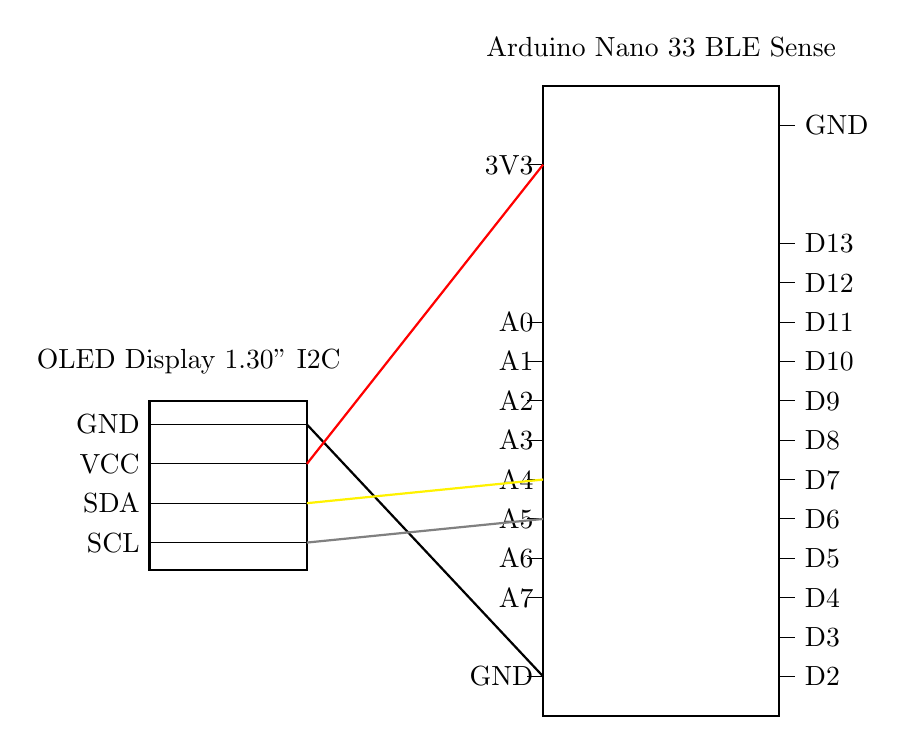
\begin{tikzpicture}
		% Arduino Nano 33 BLE Sense
		\node at (5.5, 8.5) {Arduino Nano 33 BLE Sense}; % Label above the Arduino
		\draw[thick] (4, 0) rectangle (7, 8);
		
		% Left side pins
		\foreach \i/\label in {0.5/GND, 1.5/A7, 2/A6, 2.5/A5, 3/A4, 3.5/A3, 4/A2, 4.5/A1, 5/A0, 7/3V3} {
			\draw (3.8, \i) -- (4, \i) node[left] {\label};
		}
		
		% Right side pins
		\foreach \i/\label in {0.5/D2, 1/D3, 1.5/D4, 2/D5, 2.5/D6, 3/D7, 3.5/D8, 4/D9, 4.5/D10, 5/D11, 5.5/D12, 6/D13, 7.5/GND} {
			\draw (7, \i) -- (7.2, \i) node[right] {\label};
		}
		
		% OLED Display
		\node at (-0.5, 4.5) {OLED Display 1.30'' I2C}; % Label above the OLED display
		\draw[thick] (-1, 1.85) rectangle (1, 4);
		
		% OLED pin labels on the left, pins on the right
		\foreach \i/\label in {2.2/SCL, 2.7/SDA, 3.2/VCC, 3.7/GND} {
			\draw (-1, \i) node[left] {\label} -- (1, \i);
		}
		
		% Connections
		\draw[thick, black] (4, 0.5) -- (1, 3.7); % GND to GND
		\draw[thick, red] (4, 7) -- (1, 3.2); % 3V3 to VCC
		\draw[thick, yellow] (4, 3) -- (1, 2.7); % A4 to SDA
		\draw[thick, gray] (4, 2.5) -- (1, 2.2); % A5 to SCL
		
	\end{tikzpicture}
	\captionof{figure}{Circuit diagram for connecting the Arduino Nano 33 BLE Sense with a 1.30” IIC OLED display.}
	\label{fig:OLEDCircuit}
\end{center}

 Use a laptop or computer to open the \texttt{ApplicationAPDS9960} code in the Arduino IDE. Before uploading the code, enter the \texttt{maxRed}, \texttt{maxGreen}, and \texttt{maxBlue} calibration values to ensure accurate color detection by the machine.

Once the Arduino is programmed, the color detection machine can start. Place an object approximately one centimeter in front of the APDS-9960 sensor on the Arduino. The OLED display will show important instructions and display detected colors. Each time an object is removed and replaced, the sensor will read the color in its usual interval. Ensure proper lighting, and calibrate the sensor under the same conditions in which it will operate.

\subsection{Code Explanation}
The following section provides an explanation of the application code:

\smallskip

The first part of the code initializes the Arduino Nano 33 BLE Sense with the APDS-9960 sensor and the 1.30" IIC OLED display. It includes pre-determined calibration values for red, green, and blue (\texttt{maxRed}, \texttt{maxGreen}, \texttt{maxBlue}) as integer values. In the \texttt{setup()} function, it starts serial communication, sets the LED pin as an output, and initializes the APDS-9960 sensor, printing an error message if the initialization fails. It also sets up the OLED display to show an "INITIALIZING!" message. Afterward, the LED blinks three times to indicate that the setup is complete, and the display is cleared.

\lstinputlisting[firstline=1,lastline=52]{../../Code/Nano33BLESense/Test/ApplicationAPDS9960.ino}

In the following \texttt{loop()} function, the code displays a "READY" message on the OLED display and then sets a timeout of 1000 ms to wait for color data to become available, decrementing the timeout in steps of 5 ms. If color data is not available within the timeout, a "Color measurement timeout" message is printed in the serial monitor, and the function returns. The code then resets the timeout to 1000 ms and similarly waits for proximity data. If proximity data does not become available within the timeout, a "Proximity measurement timeout" message is printed, and the function returns.

\lstinputlisting[firstline=53,lastline=81]{../../Code/Nano33BLESense/Test/ApplicationAPDS9960.ino}

In the next section of the \texttt{loop()} function, the code reads the proximity value using \texttt{APDS.readProximity()}. If a valid proximity value is detected, it prints the proximity value to the serial monitor. If the proximity value is below a specified threshold (indicating an object is close), the OLED display is cleared, and the LED is turned on as a visual indication. To capture accurate color data, all LEDs are turned on to emit white light, and multiple color readings are averaged.

The red, green, and blue color values are then mapped to a 0-255 range using predefined calibration values (\texttt{maxRed}, \texttt{maxGreen}, \texttt{maxBlue}) and are constrained within the 0-255 range. The dominant color is determined based on the highest value among red, green, and blue, and the result is displayed on the OLED. If no object is detected within the proximity threshold, a message prompts the user to hold an object near the sensor or change its position.

If the proximity reading fails, an error message is displayed on the OLED. After processing, the code turns off the LED and resets the RGB LEDs to an off state.

\lstinputlisting[firstline=83,lastline=174]{../../Code/Nano33BLESense/Test/ApplicationAPDS9960.ino}

\subsection{Application Test}

The color recognition machine reliably identifies the colors red, green, and blue from the standardized color chart. After calibration, it can also recognize other colors like light blue, yellow-green, or orange as red, green, and blue. This flexibility ensures that objects do not need to be perfectly red, green, or blue to be detected. Activating the white LED when an object approaches proves to be very practical, as it serves as a feedback mechanism alongside the OLED display, indicating to the user that color recognition is now in progress.

\subsection{Improvement Suggestions}

A key improvement would be to integrate the color recognition machine into a stable, standalone setup, so it does not need to be handheld, allowing objects to be fixed in place in front of the sensor. This would eliminate potential issues like hand movement artifacts during detection.

Another enhancement would be to equip the device with a battery, enabling portable, laptop-free operation. To conserve battery life, the white LED is deliberately programmed to illuminate only during color measurement. 

In an industrial application, adequate lighting should be ensured, potentially by adding external lighting that could be integrated into the code or kept continuously on. For use in dusty or humid environments, a thin protective cover over the sensor could prevent damage or contamination, allowing for easy cleaning or replacement as needed.

\section{Further Readings}

\begin{itemize}
	\item S. Grzesik, R. Kluwak, and B. Plikusinski, "Multispectral Sensor Application Possibility Research for Temperature Measurement," \textit{2023 23rd International Conference on Mechatronics - Mechatronika (ME)}, Brno, Czech Republic, pp. 1-6, 2023. Available at: \url{https://ieeexplore.ieee.org/document/10349583}
	
	\item SparkFun Electronics, "APDS-9960 RGB and Gesture Sensor Hookup Guide." A comprehensive guide that explains the functionality of the APDS-9960 and provides step-by-step instructions for implementation. Available at: \url{https://learn.sparkfun.com/tutorials/apds-9960-rgb-and-gesture-sensor-hookup-guide/all}
	
	\item Maker Guides, "APDS-9960 Gesture and Color Sensor with Arduino." This tutorial provides a hands-on introduction to using the APDS-9960 sensor with Arduino, including gesture and color recognition. Available at: \url{https://www.makerguides.com/apds-9960-gesture-and-color-sensor-with-arduino/}
\end{itemize}
